% 问题一
\section{问题一：单点往返最大安全载荷与货箱组批}
\label{sec:p1}

\subsection{问题分析}

问题一包含两层任务，其一是对每类运输无人机到各服务区的单点往返任务，在满足
飞行时间、载荷能耗与返航安全余量约束下求最大安全载荷；其二是依据该载荷及各
服务区货箱的质量、体积与时限，把货箱分组为架次，使总架次数与总能耗最小。
核心在于建立可核验的载荷、能耗、返航荷电状态映射：载荷越大，等效航程越短、
单位里程能耗越高，架次能耗随之上升，因此最大安全载荷由质量上限、体积上限与
能量上限三者中的最紧者决定。

\subsection{模型建立}

\subsubsection{飞行时间模型}

对航线 O01 到服务区再到 O01 的往返，设航段水平距离 $d$（按大圆距离计算），
航线最高地面高程与起飞点地面高程之差为 $h^+$，返回段下降高度为 $h^-$，
单架次飞行时间按式 \eqref{eq:time} 计算。

\begin{equation}
t_{\mathrm{fly}}= \frac{h^+}{v_{\mathrm{up}}} + \frac{d}{v_c}
+ \frac{h^-}{v_{\mathrm{down}}}
\label{eq:time}
\end{equation}

其中巡航高度为 $h_{\mathrm{cruise}}=\max_{x\in leg}\mathrm{DEM}(x)+50$\,m，
作业高度取服务区地面高程，投递悬停 30\,s。

\subsubsection{能耗模型}

按题目统一规则，水平飞行能耗由等效航程函数折算，等效航程按式
\eqref{eq:lg} 计算。

\begin{equation}
L_g(q) = L_0 - (L_0 - L_F)\left(\frac{q}{Q}\right)^{1.5}
\label{eq:lg}
\end{equation}

水平能耗为 $E_{\mathrm{hor}} = E_{\mathrm{use}}\cdot d/L_g(q)$；爬升段能耗按式
\eqref{eq:eup} 计算。

\begin{equation}
E_{\mathrm{up}} = \frac{(m_0+q)\,g\,h^+}{\eta\cdot 3.6\times10^6}\ \mathrm{kWh}
\label{eq:eup}
\end{equation}

单架次总能耗为水平能耗与爬升能耗之和，返航安全约束按式 \eqref{eq:cap}
给出，其中安全余量 $\rho=20\%$。

\begin{equation}
E_{\mathrm{total}} \le (1-\rho)\,E_{\mathrm{use}},\qquad \rho=20\%
\label{eq:cap}
\end{equation}

同时受载荷与货舱体积约束，即 $q\le Q_m$、$\sum V \le V_{\max}$。

图 \ref{fig:lgcurve} 左图给出三类机型的等效航程随载荷收缩的曲线，右图给出
三机型到 S008 往返的能耗随载荷变化，水平虚线为各自的返航安全上限，交点即
能量约束下的最大安全载荷，可见 C 型因满载航程收缩最快而最先触及上限。

\begin{figure}[htbp]
\centering
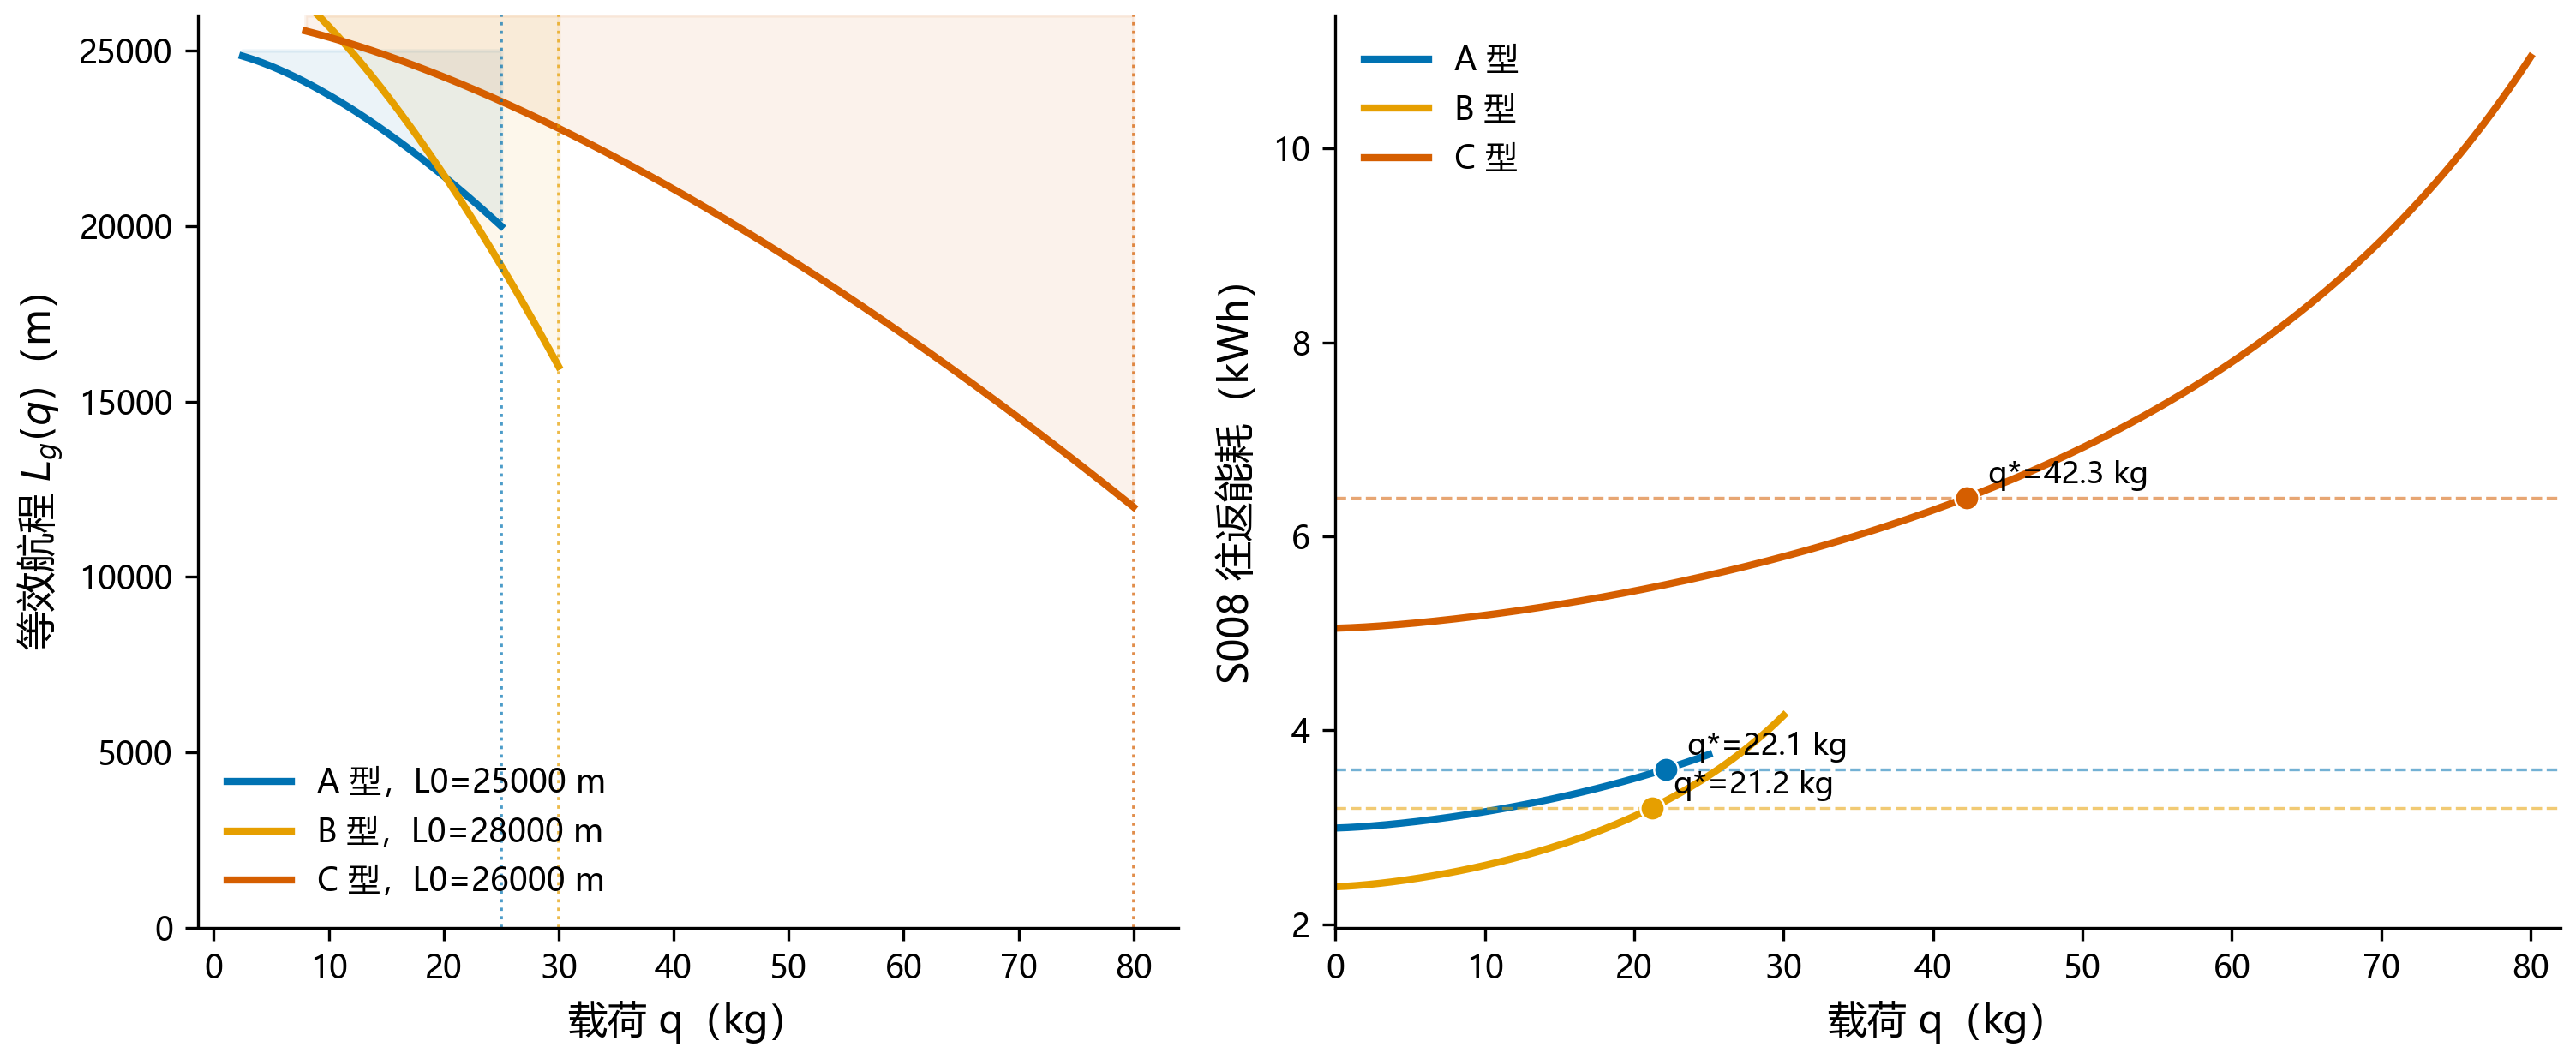
\includegraphics[width=0.96\textwidth]{figures/p1_lg_curve.png}
\caption{左：等效航程随载荷收缩曲线；右：三机型到 S008 往返能耗随载荷变化及能量上限交点}
\label{fig:lgcurve}
\end{figure}

\subsubsection{最大安全载荷求解}

对机型 $m$ 与服务区 $S_i$，总能耗随载荷 $q$ 单调递增，原因是等效航程随
$q$ 递减且爬升功递增。在可行区间内对 $q$ 二分求解
$E_{\mathrm{total}}(q)=(1-\rho)E_{\mathrm{use}}$，即得能量限制载荷，再与
质量上限、体积上限取最小，得到最大安全载荷 $q^*_{m,i}$。

\subsubsection{货箱组批模型}

各服务区货箱按机型与服务区分组，组批视为带容量约束的装箱问题：同一服务区
同一机型的货箱，按质量、体积与能耗装入最少架次，每架次往返于 O01 与单一
服务区。目标为最小化总架次数与总能耗，按式 \eqref{eq:bin} 表述。

\begin{equation}
\min \ \sum_{m,i} n_{m,i}, \qquad
\min \ \sum_{m,i}\sum_{k=1}^{n_{m,i}} E^{(k)}_{m,i}
\label{eq:bin}
\end{equation}

约束为每箱恰入一架次、架次质量体积能耗不超限、架次载荷不超过对应最大安全
载荷。

\subsection{模型求解}

对 A、B、C 三类机型逐区求最大安全载荷，结果如表 \ref{tab:qstar} 所示，其中
能量受限值用粗体标出，其余为质量或体积上限。A 型全部区域取质量上限 25\,kg；
B 型除 S008 因远距高差受能量约束降为约 28.9\,kg 外均取 30\,kg；C 型多数区域
取 80\,kg，而 S002、S003、S004、S008、S012 五个区域因航线较长或爬升较高，
受能量约束为 59.2 至 69.0\,kg。图 \ref{fig:qstar} 直观给出三机型各区域的载荷
对比，可见能量约束集中在 C 型远区。

\begin{table}[htbp]
\centering
\caption{各机型到各服务区的最大安全载荷（kg）}
\label{tab:qstar}
\resizebox{\textwidth}{!}{%
\begin{tabular}{l|ccccccccccccccc|c}
\toprule
机型 & S001 & S002 & S003 & S004 & S005 & S006 & S007 & S008 & S009 & S010 & S011 & S012 & S013 & S014 & S015 \\
\midrule
A & 25 & 25 & 25 & 25 & 25 & 25 & 25 & 25 & 25 & 25 & 25 & 25 & 25 & 25 & 25 \\
B & 30 & 30 & 30 & 30 & 30 & 30 & 30 & \textbf{28.9} & 30 & 30 & 30 & 30 & 30 & 30 & 30 \\
C & 80 & \textbf{69.0} & \textbf{68.4} & \textbf{63.9} & 80 & 80 & 80 & \textbf{59.2} & 80 & 80 & 80 & \textbf{68.2} & 80 & 80 & 80 \\
\bottomrule
\end{tabular}}
\end{table}

\begin{figure}[htbp]
\centering
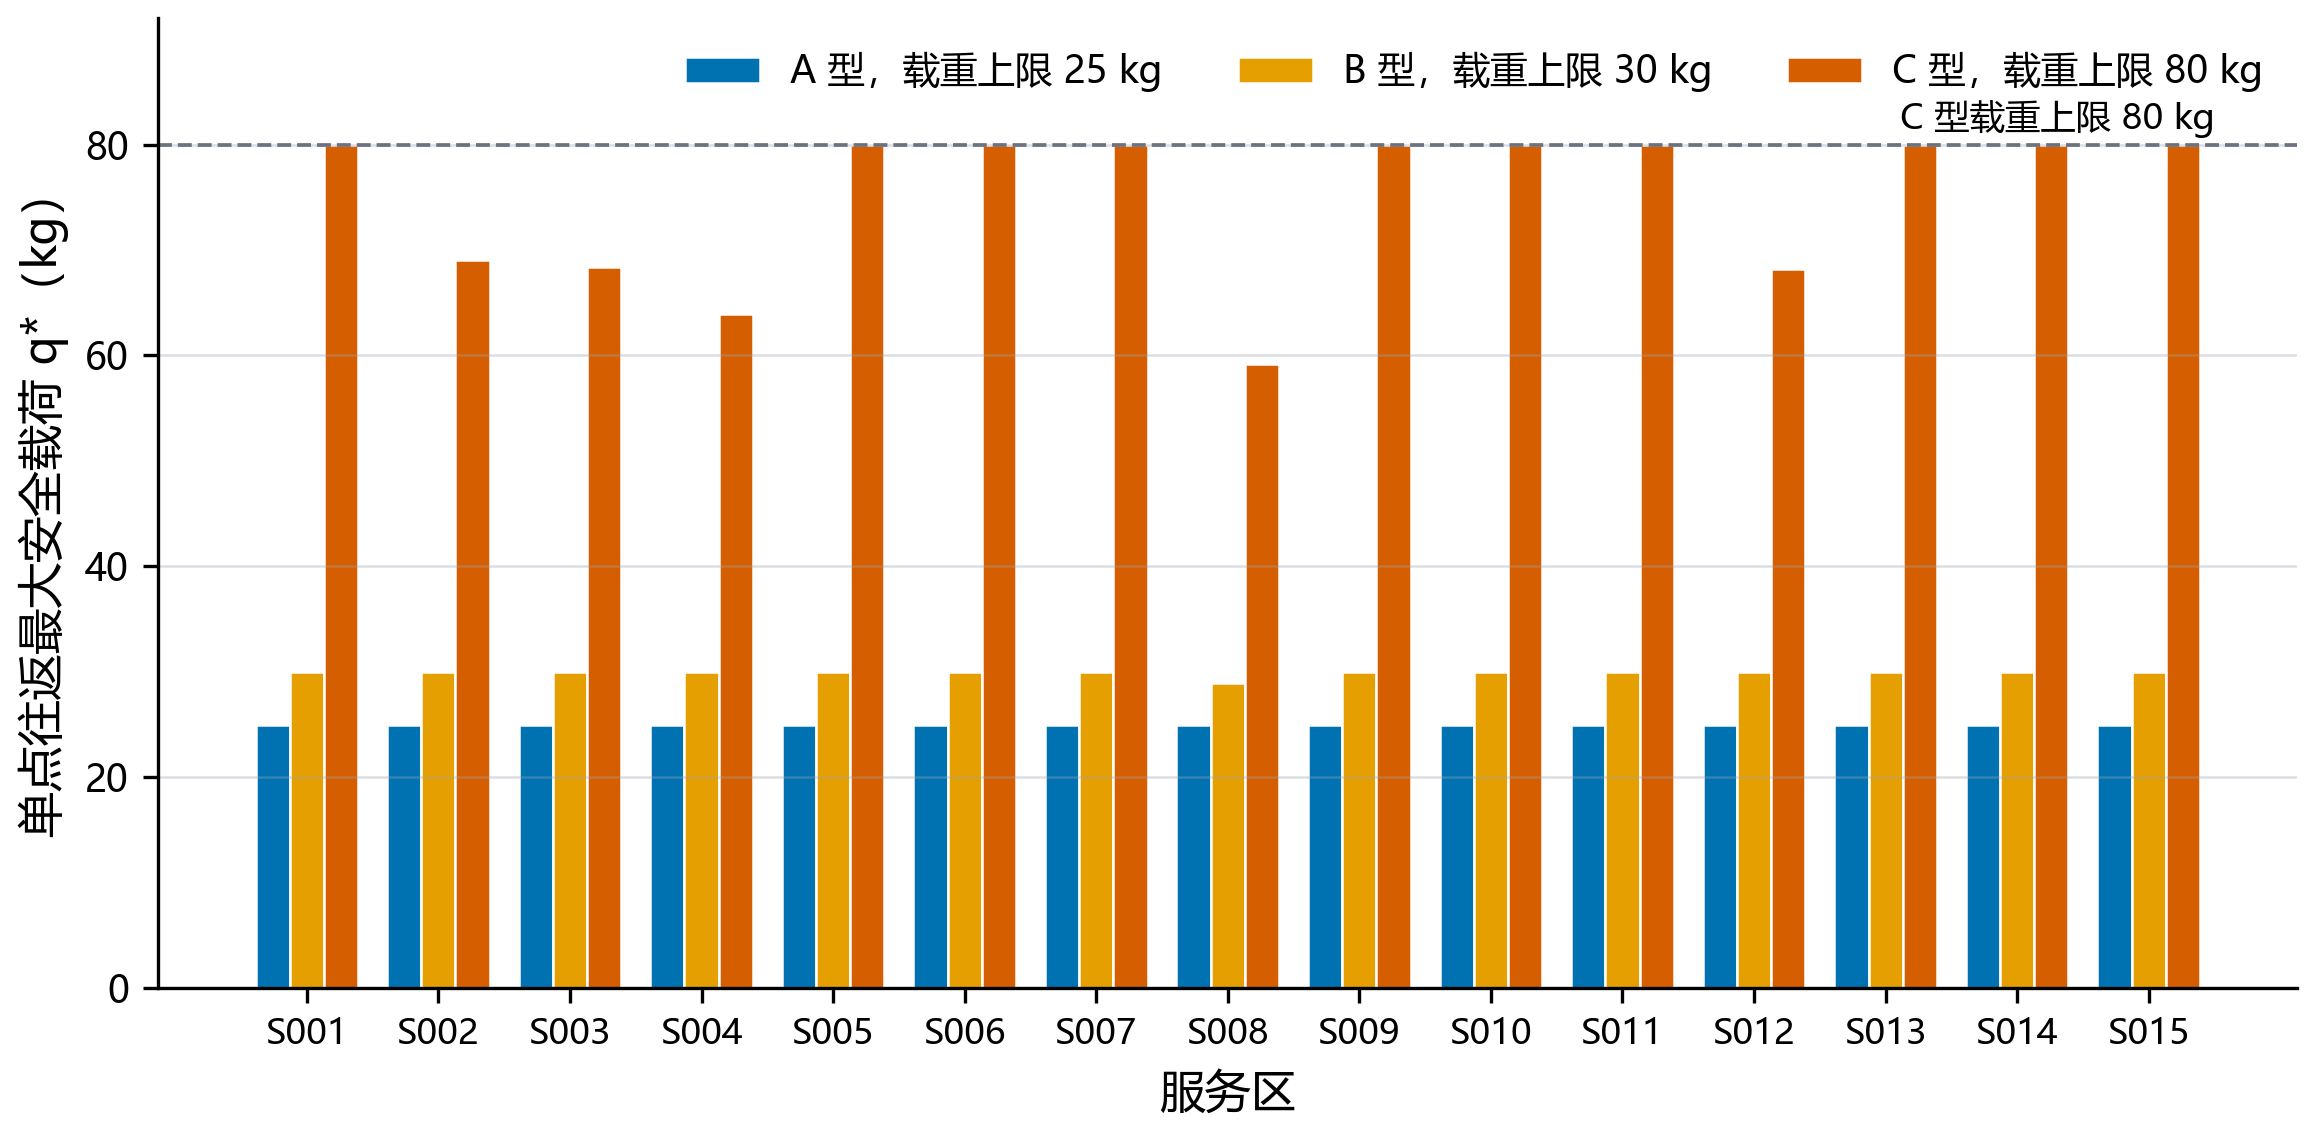
\includegraphics[width=0.84\textwidth]{figures/p1_qstar.png}
\caption{三机型在各服务区的最大安全载荷对比}
\label{fig:qstar}
\end{figure}

按式 \eqref{eq:bin} 组批，全网共 18 架次、总能耗 59.02\,kWh、总飞行时间约
32661\,s。表 \ref{tab:p1summary} 给出各服务区的组批概览：重载区由 C 型承担，
其中 S001 的 154\,kg 货箱分 2 架次完成；S009 至 S015 各 25\,kg 由 B 型单架次
送达。每架次的货箱编号、质量、体积、往返时间、能耗与返航荷电状态见《结果提交
模板》Q1 工作表；全部架次返航荷电状态均不低于 20\%，满足安全约束。

\begin{table}[htbp]
\centering
\caption{问题一各服务区组批概览}
\label{tab:p1summary}
\begin{tabular}{lcccc}
\toprule
服务区 & 货箱数 & 总质量(kg) & 架次数 & 能耗(kWh) \\
\midrule
S001 & 15 & 154 & 2 & 5.90 \\
S002 & 8 & 81 & 2 & 8.42 \\
S003 & 8 & 81 & 2 & 8.53 \\
S004 & 6 & 59 & 1 & 6.14 \\
S005--S008 & 22 & 208 & 4 & 16.03 \\
S009--S015 & 21 & 175 & 7 & 14.00 \\
\midrule
合计 & 80 & 758 & 18 & 59.02 \\
\bottomrule
\end{tabular}
\end{table}

图 \ref{fig:soc} 给出各架次按能耗升序的返航荷电状态，全部位于 20\% 安全
下限之上，最低约 23\%；重载 C 型架次能耗占比最高，返航荷电状态贴近下限，
其余架次保留更充分的余量。

\begin{figure}[htbp]
\centering
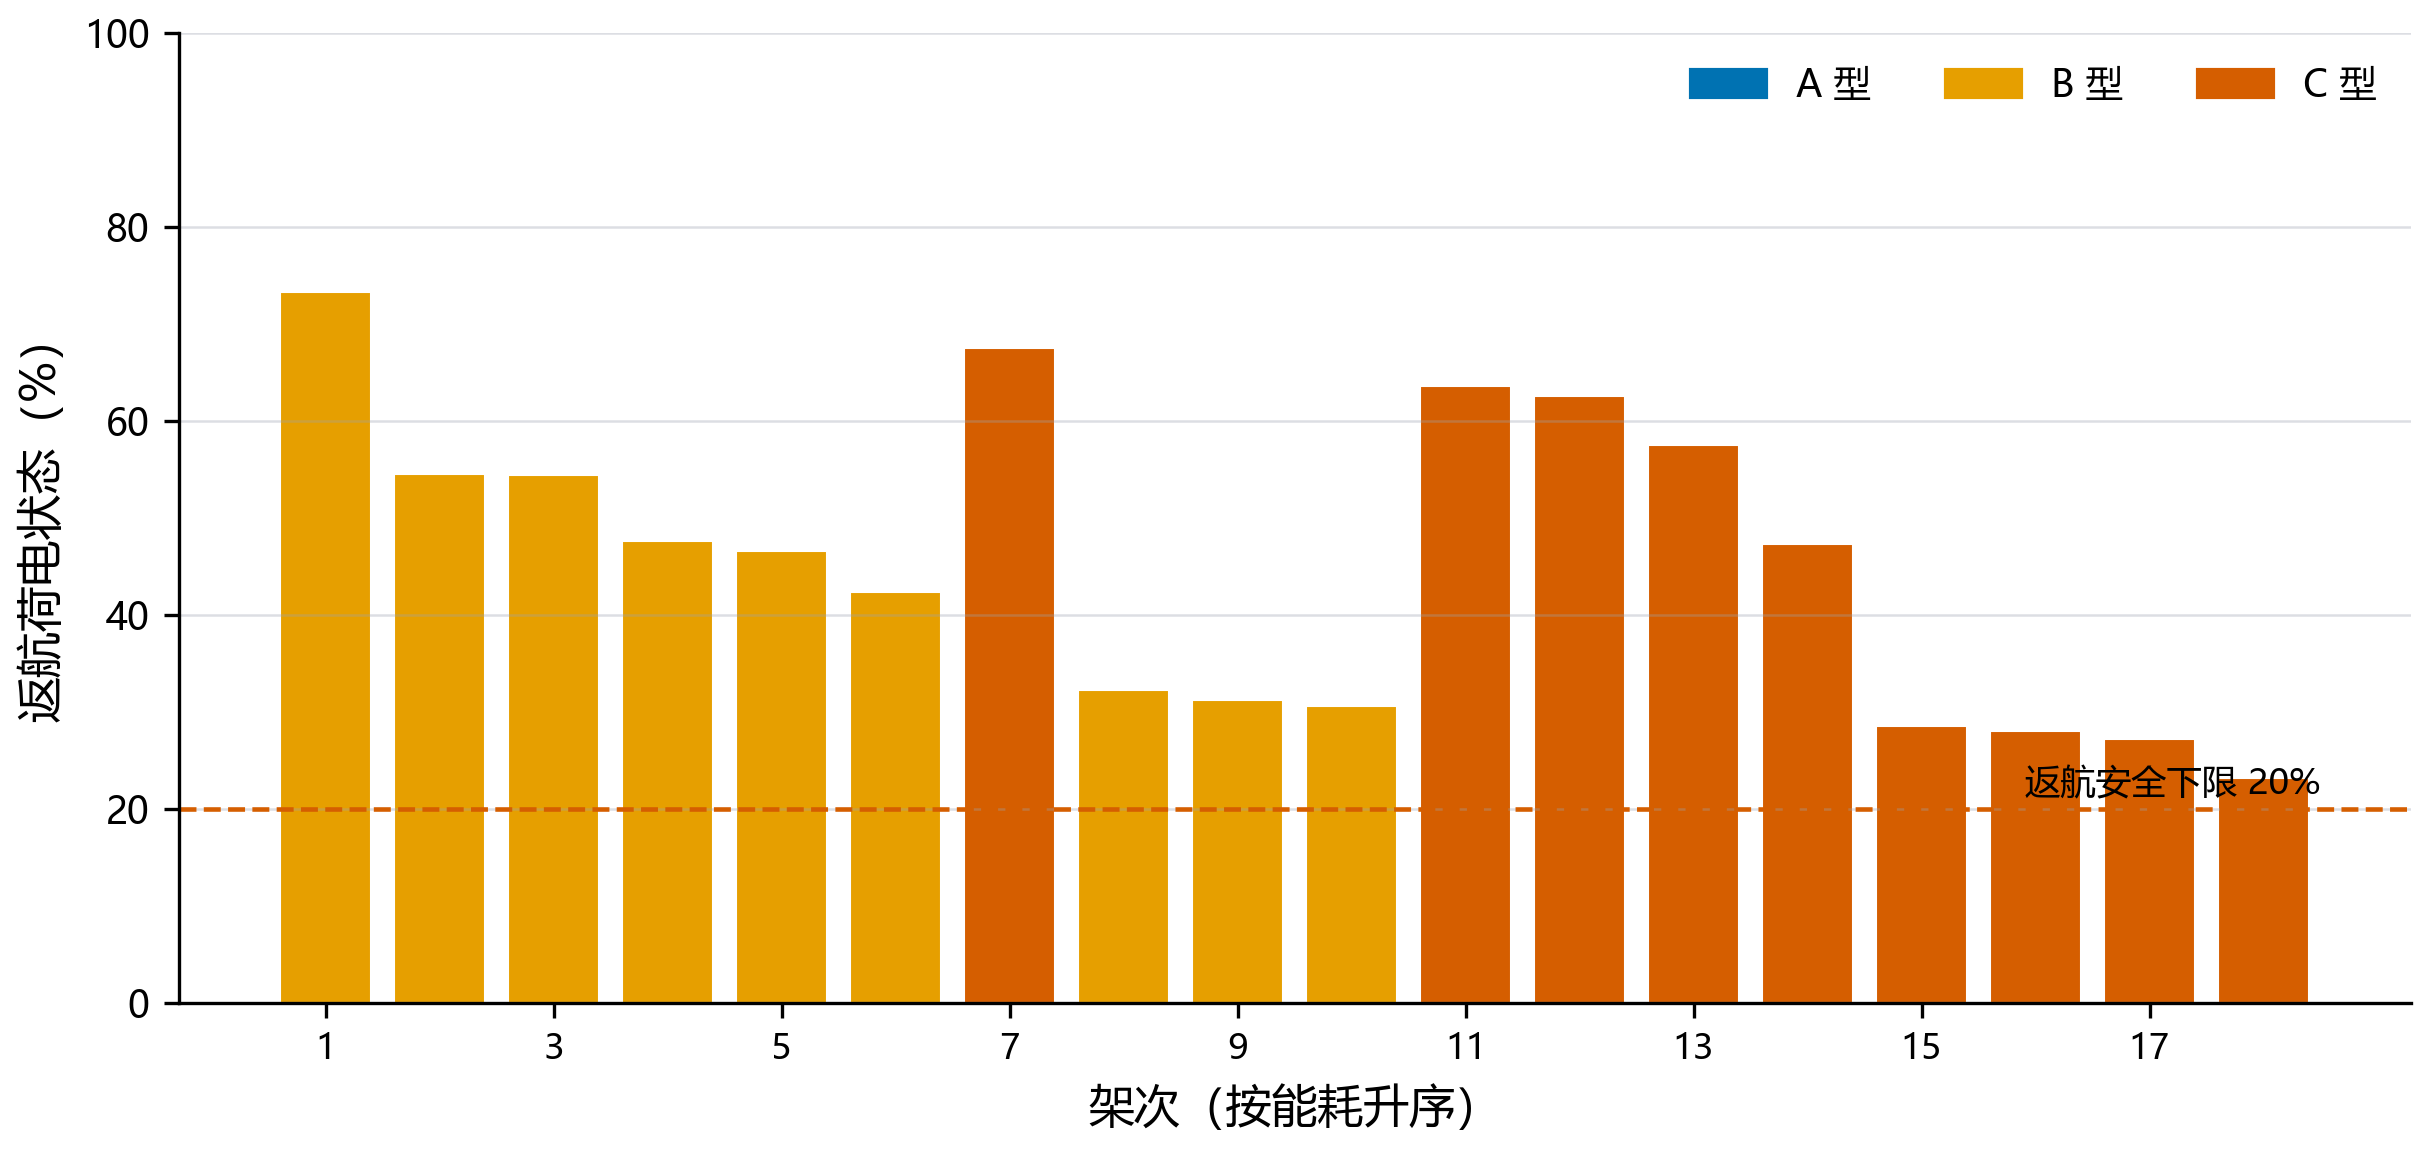
\includegraphics[width=0.9\textwidth]{figures/p1_soc.png}
\caption{问题一各架次返航荷电状态（虚线为 20\% 安全下限）}
\label{fig:soc}
\end{figure}

\subsection{结果分析}

\begin{enumerate}
\item \textbf{能量约束主导远区}：C 型到 S008 的最大安全载荷 59.2\,kg 为全网
最低，对应最长航线与最大爬升的组合；A、B 型因质量上限较低，能量约束几乎不
生效，仅 B 型到 S008 略受约束。这说明远距加高差是山区无人机投送的关键瓶颈。
\item \textbf{组批节省架次}：重载区用 C 型多装，单架 63.9 至 80\,kg，轻载区用
B 型单架直送，18 架次即完成全部 80 箱，架次利用率较高。
\item \textbf{安全余量与效率权衡}：安全余量比例 $\rho$ 从 0.2 增大到 0.35 时，
架次数由 18 增至 25，能耗由 59.02 升至 77.63\,kWh，增幅约 31.5%；$\rho$ 由
0.35 增至 0.40 时架次数不变而能耗由 77.63 降至 74.62\,kWh，说明该区间发生
机型结构切换，部分 C 型远区架次改由更经济的组合完成。详细的扫描结果见第
\ref{sec:sens}节。
\end{enumerate}